
\section{ChatGPT suitability evaluation}\label{sec:metric_based_eval}

As the first experiment shows the limitations of ChatGPT while detecting and refactoring data clump, these results center on human feedback which is subject to bias and other uncontrollable influences. 

To further evaluate the usefulness of ChatGPT in the pipeline, a second experiment was conducted.

In this second experiment, tests were conducted to assess the suitability of ChatGPT performing steps of the pipeline. In contrast of the first experiment, this experiment is centered on a limited set of projects and uses more metrics while leaving out human feedback. 

In total four experiments (numbered from 2A to 2D) have been conducted where each experiment can be read separately from the other.

\subsection{General methodology}

In contrast to the feedback-driven experiment, multiple data clumps are selected that will be used in the succeeding steps. These data clumps are not chosen manually as in the first experiment but selected via an algorithm. This algorithm is as follows:
\begin{enumerate}
    \item Select 
\textit{n}
 data clumps based on one criterion, and 
\textit{n}
 data clumps based on another criterion, and so forth
    \item Determine the total file size of the files affected by this set of data clump
    \item Save this set of data clumps if its file size is smaller than the current minimum
    \item if the current minimum has not improved for 1000 iterations, return the minimum and the associated data clumps
\end{enumerate}

With this local optimum search strategy, a set of data clumps is retrieved that can be used as the basis for the detection, filtering and refactoring step while also minimizing the total file size transmitted to the \ac{LLM}. 

The exact criteria and amount of data clumps used for the data clump selection depend on the concrete experiment. For instance, if the best data clump should be chosen by the model, very large data clumps and data clumps affecting many classes and methods should be transmitted. This creates a stark contrast between the proposed data clumps and forces the model to make a genuine selection for a suitable data clump. In the refactoring step only two random data clumps are considered  because it can be expected that subsequent validation steps would increase the amount of transmitted data even more, so that submitting more files would increase the likelihood of context window overflow. This issue does not occur under the detection and filtering step. 

\subsubsection{Selection of projects}

Selecting projects for this experiment is easier because no human feedback is required so that the active maintaining criterion in section \ref{sec:github_projects} is not relevant. However, the other criteria are still relevant. 

As a result, projects were selected that have already been used for experiment regarding code smells or refactoring in the literature. These include:
\begin{description}
    \item[ArgoUML] The leading open source UML modeling tool
    \item[RocketMQ] A cloud-native messaging, eventing, streaming real-time data processing platform
    \item[Dolphinscheduler] A distributed and extensible open-source workflow orchestration platform
\end{description}


\subsubsection{Parameterization}

One aspect important to consider while using \acp{LLM} is the existence of parameters that can be adjusted. These parameters determine how the model can interpret the instruction and how it should respond. Using different hyper-parameters can show whether special care should be given to these parameters or whether they are irrelevant. The following parameters are considered: 

\begin{description}
	\item [Temperature] This parameter describes the randomness of the output of the model. The less temperature, the more the output is predictable. However, this reduces the model's potential for creating creative output.
	
	\item[Instruction type] This parameter describes how the concept of data clump is taught to the model. Three types are tested: In the definition-based approach a formal definition resembling the definition given in section \ref{sec:data_clump_def} is provided. In contrast using the no-definition method, the term \enquote{data clump} is not explained at all so that the model must use its inherent knowledge. A third option is to provide examples of data clumps In Java which requires the model to learn this concept by analyzing similairities in source code.  
	
	\item [Input type] This parameter is discussed in section \ref{sec:input_format}. The available values for this parameter depends in what steps of the pipeline the model is used. For instance, in the detection step, the data clump type context is not available and cannot be submitted to the model. In the refactoring step, only source code can be submitted as that source code must be changed by the model.
	
	\item [Margin] This parameter is only relevant if code snippets are transmitted. In other cases, it would have no effect since it only affect the size of the code snipptes. Values considered here are 0, 1, 2, 5 and 10, 
	
	
\end{description}

Other parameters that could be considered are the model, which has a great impact on the output, the output format, the specific model, and the concrete instruction given to the model. However varying too many parameters can be a significant obstacle in evaluation experiments so that only these parameters are used. 

\subsubsection{Threats to validity}

These experiments have their limitations too. 

In the detection experiment, the returned data clump type context is linked to the real data clump type context to determine which data clumps are detected. The metric finds the real data clump that shares the most similarities with the returned data clump. However, this could be a complete wrong data clump. For instance, if the model returns a correct class name containing a data clump but otherwise is wrong, it is still considered for the data clump type, size, and occurrence metric. The accuracy of the information is only considered in the surety metric.

Additionally for the output accuracy metric, the relevance of each parameter in data clump type context is disregarded. For instance, the data clump type context contains information about the line number of each data clump. Even if this information is missing, it can be replaced by considering the other information ( variable names, method name, class name). Hence, the potential impact false information has on the refactoring step has is ignored. 





\subsubsection{Metrics}

To evaluate the quality of \ac{LLM} in the pipeline, several metrics are employed that give an hindsight about the potential of such models. These metrics return a numerical value.  A larger value is deemed better than a low value. However, these metrics are not scaled to a uniform range. The metrics can be further categorized into common metrics and experiment-specific metrics. 

Common metrics are used by each experiment as they are not specific to a specific experiments and can be evaluated by all experiments. These metrics include
\begin{description}
    \item [Price] The total price of a query which includes the price for processing the input and the price for the output
    \item [Time] The time needed from sending the query to the \ac{LLM} server until it responds. 
    \item[ Data-clump-specific] Attributes of the data clump considered by the model. This includes the size, occurrence, affected files of the respective data clump. 
    \item[Validity of the JSON] This metrics determines whether the output of the \ac{LLM} is valid \ac{JSON}. Invalid output can occur if the model hallucinates or the output is too large.
\end{description}


On the other hand, experiment-specific metrics do only apply to a specific experiment and would not make sense for all experiments. These metrics are in the subsections for each individual test. 


\subsection{Experiment 2A: Data clump detection}

Detecting data clumps is an essential part to refactor them. Because it happens at a very early state in the pipeline, it is even more important that the data clump detection data is accurate and conforms to the specification. The question is here is whether the model can perform this task so that subsequent steps of the pipeline (e.~g. a manual refactoring tool) can rely on the data. If the reliability of the results is too low, it becomes more challenging to develop manual that can handle with possibly erroneous data.

Additionally, in contrast to a manual tool, detecting data clumps via  a model might also include a filtering process because the model might not return all data clumps but only a subset of them. This means that further filtering in subsequent steps might not be necessary. 

The format presented in appendix \ref{app:data_clump_format} is used as the output format because subsequent handlers have been adapted on this context. 


\subsubsection{Methodology}

For this experiment, either code snippets or complete files are submitted, and the model is asked to find all data clumps and to report its result in the specified format.
Because transmitting the full project is infeasible, the data clumps are previously detected using the \textit{DataClumpDoctor}. The relevant locations of the most important data clumps are then used as a basis to submit the request to the model. In case of code snippets, this would mean that the code snippets only contain data clumps and no other parts of the source code. As this might induce a bias, all other methods in the respective file having at least three parameters are included too. Also all fields in a class are submitted if such class has at least three fields. As a result, the model still has to identify the correct data clump while  the transmitted tokens are minimized.  


The following metrics are used for evaluating this tests:

\begin{description}
    \item[Sensitivity and specificity] These describe the false negative and false positive rate of the detection. The model might miss a data clump so that it is not reported (false negative). It might also report  a data clump that is not detected as a data clump by the \textit{DataClumpDoctor}. In the latter case, cautiousness is warranted as the \ac{LLM} can detect more data clumps than a traditional algorithm. 

    \item[Correctness of output format]

    As already noted, the correctness of the output format representing the data clump is essential. If the model reports in wrong format, the data must be interpreted again which increases the risk of faults complicates integrating the \ac{LLM}

    \item [Surety of the results] In contrast to the preceding metric, not the exact output format is analyzed but the correctness of the entailed data. For instance, the model might return a wrong line number or method name which would have a significant impact on succeeding steps. 

    

   
\end{description}

\subsubsection{Threats to validity}

In the detection experiment, the returned data clump type context is linked to the real data clump type context to determine which data clumps are detected. The metric finds the real data clump that shares the most similarities with the returned data clump. However, this could be a complete wrong data clump. For instance, if the model returns a correct class name containing a data clump but otherwise is wrong, it is still considered for the data clump type, size, and occurrence metric. The accuracy of the information is only considered in the surety metric.

Additionally for the output accuracy metric, the relevance of each parameter in data clump type context is disregarded. For instance, the data clump type context contains information about the line number of each data clump. Even if this information is missing, it can be replaced by considering the other information ( variable names, method name, class name). 

\subsubsection{Results} 

The experiment shows the limitation of the output format even with some simplifications. On average, only three data clumps are returned which is not enough to cover all data clumps in the chosen projects. This is further highlighted by the \ac{JSON} validity metric which is about 80 percent. 

Considering the effect of the temperature, the number of detected data clumps decreases with higher temperature while  the \ac{JSON} is more often valid. At the same time, the costs and the processing time decreases because fewer token are output. There is an inconclusive effect of the temperature on the surety. The surety decreases with rising temperature for \textit{RocketMQ} and \textit{Dolphinscheduler} while it increases in the case of \textit{ArgoUML}. 

The effect of the input type is also visible. Providing full files instead of code snippets decreases the surety massively. For instance,  the surety for for \textit{ArgoUML} in the case of full files is -4.16 while it is 2.31 in the code snippets case. Considering the price, the full file approach always cost more but the extent differs sharply between the projects. 

Changing the margin leads to very inconclusive results per project. \textit{ArgoUML} and \textit{Dolphinscheduler} have a higher surety if the margin is larger, which is not the case for \textit{RocketMQ}. However, there is a steady increase in the cost for higher margins for all projects


\subsection{Experiment 2B data clump detection with modification}

This experiment is a derivation from the preceding one. Similarly to the detection experiment, the goal is to detect data clumps in a software project.

However, now the source code is modified to test whether the model can detect data clumps that the \textit{DataClumpDoctor} would not be able to detect because the names or the types of at least one data clump item is different. Three types of modification should be distinguished:

\begin{description}
    \item[Synonym] A synonym of variable name is used. For instance, the words \textit{change} and \textit{modification} have a very similar  meaning. 

    \item[ Typographical error] A spelling error resulting in a slightly modified name. This could be caused by a developer not knowing the exact spelling of a word. However, it could also happen by accident if the developer mistypes while writing the source code.

    \item [Type mismatch] Two variables that share the exact names but have a similar type 
\end{description}

In each of these cases, it can be argued that a data clump can still exist even with these modifications. For synonyms and type mismatches however, allowing such changes might decrease the specificity of the detection because they might be purpose and cannot be easily refactored. 

\subsubsection{Methodology}

For this experiment, data clumps with exactly three items were randomly sampled. For each data clump, one modification was introduced (e.~g. replacing the name of a variables by a synonym), if such change was reasonable.

It is important to only consider data clumps with exactly three items because  a modification of one item would invalidate the data clump for a traditional tool like the \textit{DataClumpDoctor}. If larger data clumps were to be submitted, the model could return only a subset of the data clump items and ignore the item with the modifications. 

To find synonyms for a given word, the WordNet \cite{10.7551/mitpress/7287.001.0001} library was used. This library can find similar words to a given word.

To find typographical errors, the Birbeck database \cite{birbeck} was used which contains spelling mistakes in the English language, From this database, a spelling mistakes was chosen that could reasonably happen to a developer (e.~g. writing a letter twice, omitting a letter etc.). 

Type modification were only performed on numerical types such as \textit{int}. For instance,  the type \textit{long} might be replaced by \textit{int}. 
\subsubsection{Threats of validity}
In general, the threats of validity from the detection experiment apply here too. 

Additionally, the concrete modification applied to a data clump item can strongly affect the result. For instance, the Birbeck dataset contains mostly spelling mistakes made by children or illiterate adults so that developers could possible make other mistakes. 

Also the WordNet database is not specialized on technical terms but is more general. This means that the synonyms chosen here might not be synonyms used by a developer.

\subsubsection{Results}

In summary, ChatGPT was able to detect data clumps with synonyms and typos while facing enormous challenges identifying data clumps with different types. However, the capability of ChatGPT ignoring such modifications varies strongly between projects. For instance, in \textit{Dolphinscheduler} no data clumps with synonyms are detected while typos are detected well. On the other hand, typos are generally not detected in the other projects though synonyms are.

Furthermore, there is a tendency that lower temperatures lead to a better detection of data clumps with modifications. 

Considering the input type, it appears that providing code snippets leads to better detection of synonyms. On the other hand, the detection of typos is slightly better if full code files are provided.  

The effect of the margin size is much more limited and inconclusive.

\subsection{Experiment 2C: Data clump filtering by model}

The filtering experiment is somewhat similar to the detection experiment. However, here the model is told to return one data clump that is most relevant. Additionally, it does not need to use the data clump type context as the output format because this information already exists. 

As outlined in section \ref{sec:data_clump_filtering}, there are multiple approaches for filtering data clumps, which can already be implemented manually. 
The question here is whether the \ac{LLM} uses novel filtering approaches or simply relies on the metric discussed in section \ref{sec:data_clump_filtering}. In the latter case, it is more useful to use the manual algorithm because they are reliable and do not incur the costs associated with Large Language Models. 

\subsubsection{Methodology}

This experiment is conducted similarly to the detection test. However, at this time, the data clump type context as outlined in appendix \ref{app:data_clump_format} is included as a possible input format. Additionally, if code snippets are provided, they always contain data clumps as opposed to possible data clumps as outlined in the detection experiment. 
The output format is discussed in section \ref{sec:output_format_filtering}
The following metrics are used to evaluate this experiment:
\begin{description}
    
    \item [Rank] The rank of the chosen data clump with regard to the metrics: Size, occurence, and affected files. This metric assesses whether the modekl would simply return the same data clump as a traditional metric or would return another data clump 
    \item [Accuracy] Determines  whether the returned information is sufficient to detect a single data clump. Given the best fitting data clump,  it is the ratio of the data clump properties that identify a data clump and the properties that do not belong to the data clump. 
    \item [Reason] A reason given by the model that explains why the model chose a particular data clump. 
\end{description}

\subsubsection{Threats of validity}

One threat of validity is   that only one data clumps is returned although it might make sense to return more (e.~g. three). Additionally, as a result of the similarity to the detection experiment, the flaws of the former can be flaws of the latter experiment. 
\subsubsection{Results}

\begin{figure}
    \centering
    \begin{subfigure}[b]{0.4\textwidth}
    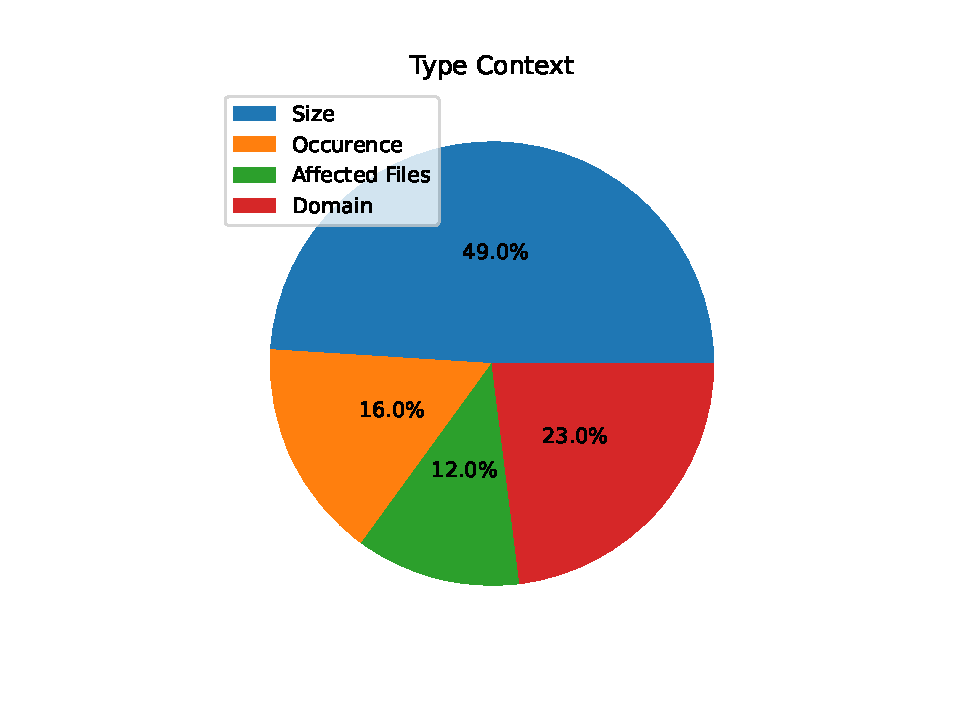
\includegraphics[width=1\columnwidth]{figures/chapter5/filter_reason_Type_Context.pdf}
     \caption{Data clump type context provided}
    \label{fig:pie_filter_data_clump_type_context}
    \end{subfigure}
        \begin{subfigure}[b]{0.4\textwidth}
    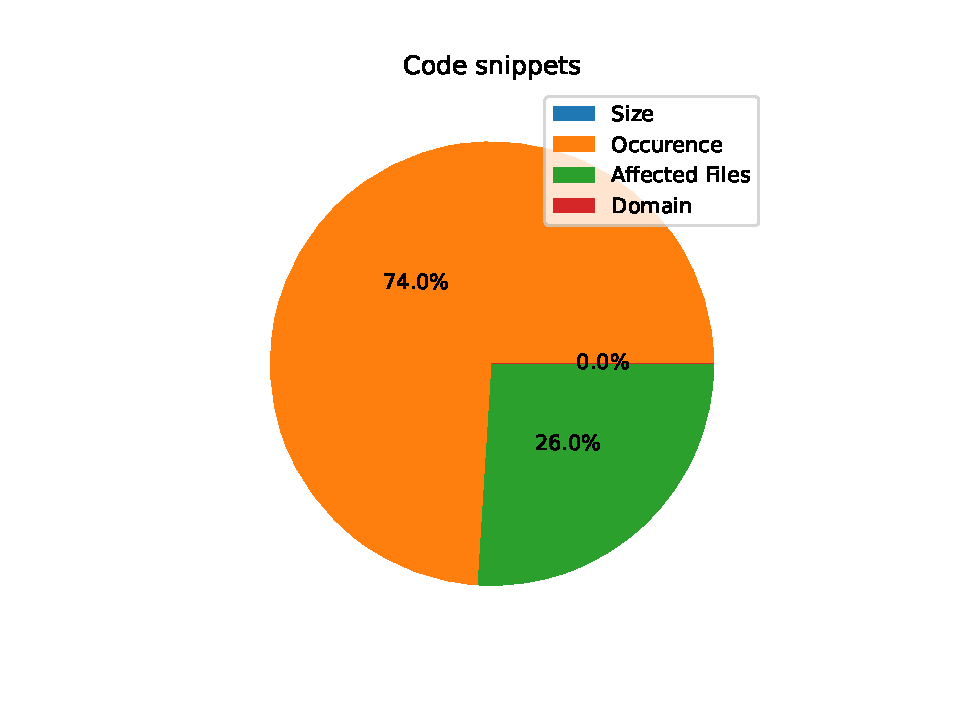
\includegraphics[width=1\columnwidth]{figures/chapter5/filter_reason_Code_snippets.pdf}
     \caption{Code snippets provided}
    \label{fig:pie_filter_code_snippets}
    \end{subfigure}
    \hspace{4cm}
           \begin{subfigure}[b]{0.4\textwidth}
    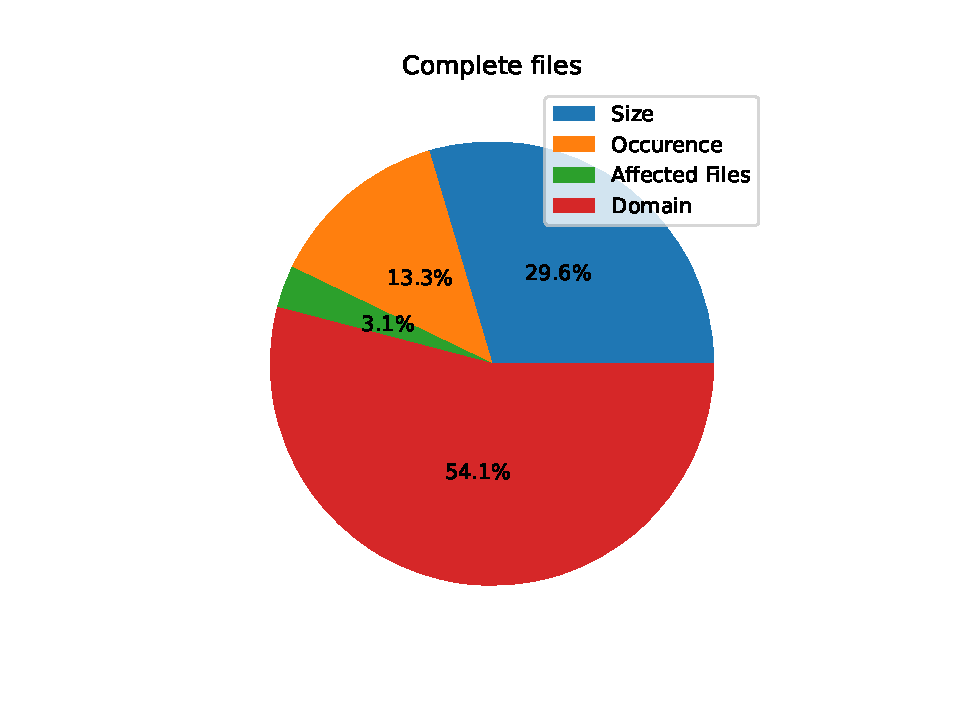
\includegraphics[width=1\columnwidth]{figures/chapter5/filter_reason_Complete_files.pdf}
     \caption{Complete files  provided}
    \label{fig:pie_filter_full_code}
    \end{subfigure}
    \caption{Distributions of reasons depending on the input format}
    \label{fig:reason_distr}
\end{figure}

Figure \ref{fig:reason_distr} shows three pie charts that visualize how the input types affect which data clump the model deems to be the most important one. 

The left-most figure \ref{fig:pie_filter_data_clump_type_context} illustrates the case if the data clump type context as described in appendix \ref{app:data_clump_format} is provided. Then, the model seems to be focused on the size of the data clump (49~\% of all instances). However, also the domain of the data clump items has a potential role (23~\% of all instances).

If code snippets are submitted, it can be seen on figure \ref{fig:pie_filter_code_snippets} that the domain and  the size of the data clumps have no influence anymore. Here, the occurrence of a data clump has a major impact as 74~\% of all reasons mentions this metric. 

Last but not least,. in the case of transmitting full source code files, the distribution again changed rapidly. As figure \ref{fig:pie_filter_full_code} depicts, the domain of the data clumps items becomes the most important aspect, while the occurrence and the affected files are less relevant.

These comparisons show that the choice of the input format can have a significant impact on how the \ac{LLM} interprets the data. Partly, there are good reasons for these distribution changes. For instance, in the code snippet cases, the occurrence and affected files metric are also transmitted to the model. Since the range of the occurrence metric is larger, the model is more likely to use the occurrence metric. Also if full source code files are provided, the model can infer the importance of a data clump better and can therefore better decide that a group of variables shares a common domain. 


\subsection{Experiment 2D: Data clump refactoring}

Evaluating how an \ac{LLM} performs data clump refactoring is another method to assess the suitability of the models for use in the pipeline. Here, especially the creativity is important. If a model merely refactors similarly to a manual tool (e.~g. IntelliJ), it has less use.

If however, the \ac{LLM} extracts more functionality by creating new methods or solves the data clump in other ways, the advantages of the model become more obvious.



\subsubsection{Methodology}

In contrast, to the detection and filtering experiment, this experiment included actual modification to the source code. 

The model is instructed to find and refactor all data clumps. 
The model outputs by providing diff instruction as discussed in section \ref{sec:output_processing} and the modifications are applied.  The modified program is tested with the respective build system (gradle or maven). if the build fails, the model is provided with error messages and the content of the affected lines, and the model is instructed to fix these issues. If after five attempts, the project still does not compiles, no further attempts are made. 

The following metrics are used for evaluating this tests:

\begin{description}
    \item [Compilation attempts] The number of attempts remaining. For instance, if the model takes four iterations to fix all compilation issues, one iteration is remaining. 
    \item[ Final program validity] Whether a refactored program is compilable at the end. 
    \item [Number of Git changes] The information obtaining by executing \textit{git diff} contains the number of inserted lines, deleted lines and added files. While the usefulness of this metric is difficult to ascertain, it shows whether the model has made excessive changes that could be deemed unnecessary. On the other hand, this could be a sign that other code smells are fixed. 
    \item [Rich class] Whether the extracted class are more than mere data classes
    \item [Over-commenting] During initial testing it was observed that the model tries to correct errors not my addressing the root cause but commenting erroneous lines out.  This behavior resembles a strategy observed by novice programmers. \cite{10.1145/1151588.1151600} This metric counts the number of commented lines before and after the refactoring to assess whether such a behavior has occurred. 
    \item [Removed data clumps] This metric assesses how many data clumps were removed during the refactoring process

    \item [Removed variables] In contrast to the removed data clump metric, this metric counts the total number of fields and parameters removed during the refactoring process
\end{description}

\subsubsection{Threats to validity}

For the refactoring experiments, several limitation should be considered. Noteworthy, the number of data clumps transmitted is severely limited as the model should also correct errors which requires retransmitting files multiple times. In many cases, this repeated transmission can exceed the context window so that the number of data clumps ( and hence in most cases the number of transmitted files)  needs to be reduced. 

Additionally, in the validation phase, the instruction to fix errors is constant, namely \enquote{Fix all errors in the respective files}. In contrast to a human in the loop who might be able to help the model to solve the compiler errors, the model can only rely on the compiler errors and the content of the files affected by these compiler errors. This can be problematic if the model returns a specific correction output but this output cannot be parsed correctly (e.~g. wrong line numbers). In that case, no compiler errors are fixed and the model might be tempted to use the same output again until the five attempts are exhausted. This problem could only be prevented if concrete feedback is given which outside of the scope of this master thesis. 

\subsubsection{Results}

In general, ChatGPT is unable to fully perform the refactoring so that the resulting program does compile and work. However it is able to remove many variables and decrease the code size. Many refactorings however are incomplete so that the data clump still remains although fewer parts of the source code are affected.

Astonishingly, ChatGPT fails to provide concrete diff instruction because 50 percent of  diff instructions cannot be interpreted which leads to no change in the source code. 

Additionally, the extracted class are seldom rich (10 percent) which indicates that generating helpful classes is possible but still limited. 

Here, also the effect of the temperature seems to be inconclusive as no trend is visible.

However, the effect of the input type is visible. Providing full code files decreases the number of valid diff instructions and leads to less removed variables. However, the number of removed data clumps is often not correlated with the number of removed variables.



As for the margin parameters, there is a strong contrast between a margin of 0 and larger margin. For instance, a margin of 0 leads to a high number of non-interpretable diff instructions. Here also, many results are inconclusive and vary between projects. 


\subsection{Discussion}

The results from all four experiments show that the effect of the parameter are very project-specific and general trends are hard to decipher. However thes show that ChatGPt is capable of being used in the pipeline and perform operations that a traditional program would be unable to do.

Further experiments needs to be conducted that anaylze thestark difference of parameter's impact om the quality of the results. The observations discussed in  \cite{hallCodeSmellsHave2014} shows a similar discrepancy with regard to data clumps per projects although there it is about the induction of faults.

Further analysis on whether there are specific project categories that cause these irregularities needs to be done. 

"It is evident that selecting suitable parameters is essential for higher quality in the refactoring pipeline. Since general trends are difficult to discern,  the selection of parameters must be performed per project.